\documentclass[10pt,a4paper]{report}
\usepackage[utf8]{inputenc}
\usepackage[russian]{babel}
\usepackage[OT1]{fontenc}
\usepackage{amsmath}
\usepackage{amsfonts}
\usepackage{amssymb}
\usepackage{graphicx}
\author{Скрипаль Борис, Баратынский Александр}
\title{Отчет по лабораторной работе по дисциплине "Сети и системы передачи данных"\newline
на тему "Визуализация сигналов во временной и частотной области"}
\date{23.02.14}
\begin{document}
\maketitle
\pagebreak
\chapter{Лабораторная работа 4}
\section{Цель работы}
Познакомиться со средствами генерации сигналов и визуализации их спектров.
\section{Постановка задачи}
В командном окне MATLAB и в среде Simulink промоделировать чистый синусоидальный сигнал, 
так же синусоидальный сигнал с шумом. Получить их спектры.
\section{Введение}
В ходе данной лабораторной работы необходимо промоделировать чистый синусоидальный сигнал, а так же синусоидальный сигнал с шумом и получить их представления во временной и частотной областях. Синусоидальный сигнал задаётся по следующей формуле: 
\begin{displaymath}
A(t) = A_0 * sin(2*\pi *f*t + u_0)
\end{displaymath}
Для создания зашумленного синусоидального сигнала, к чистому синусоидальному сигналу прибавляется случайная составляющая, по формуле:
\begin{displaymath}
A(t) = A_0 * sin(2*\pi *f*t + u_0) + A_1*rand()
\end{displaymath}
Для выделения частот регулярных составляющих сигнала необходимо использовать преобразование Фурье, реализуемое следующей формулой:
\begin{displaymath}
X(k) = \sum_{j=1}^N x(j)*e^{2*\frac{x}{N(j-1)(k-1)}}
\end{displaymath}
\section{Алгоритм работы}
\begin{itemize}
\item Построение чистого синусоидального сигнала с регулярной составляющей 10 Гц и с нулевой начальной фазой
\item Вывод временной характеристики сигнала
\item Реализация одномерного преобразования Фурье на основе 512 точек
\item Построение графика спектральной плотности для чистого синусоидального сигнала
\item Построение зашумленного синусоидального сигнала путем добавления к чистому синусоидальному сигналу случайной аддитивной компоненты с нулевым средним
\item Вывод временной характеристики полученного сигнала
\item Реализазия одномерного преобразования Фурье на основе 512 точек
\item Построение графика спектральной плотности для зашумленного синусоидального сигнала
\end{itemize}
\section{Код MATLAB}
x = 0:0.01:4*pi;\newline
t0 = 10;\newline
\%исходный сигнал\newline
ynorm = sin(2*pi*t0*x);\newline
plot(x(1:200),ynorm(1:200))\newline
grid\newline
\%спектр исходного сигнала\newline
figure\newline
spectrum = fft(ynorm,512);\newline
normspectrum = spectrum.*conj(spectrum)/512;\newline
f=100*(0:255)/512;\newline
plot(f, normspectrum(1:256))\newline
axis([0 max(f) 0 10])\newline
grid\newline
\%зашумленный сигнал\newline
ynoize = ynorm+ 0.8*rand(size(x));\newline
figure\newline
plot(x(1:200),ynoize(1:200));\newline
grid\newline
\%спектр зашумленного сигнала\newline
spectrum = fft(ynoize,512);\newline
noizespectrum = spectrum.*conj(spectrum)/512;\newline
figure\newline
plot(f, noizespectrum(1:256))\newline
axis([0 max(f) 0 10])\newline
grid\newline
\section{Результаты работы}
В результате выполнения программы мы получили четыре графика: временная и частотная характеристика для чистого и зашумленного синусоидального сигнала. Графики представленны ниже. \newpage
\begin{figure}
\begin{center}
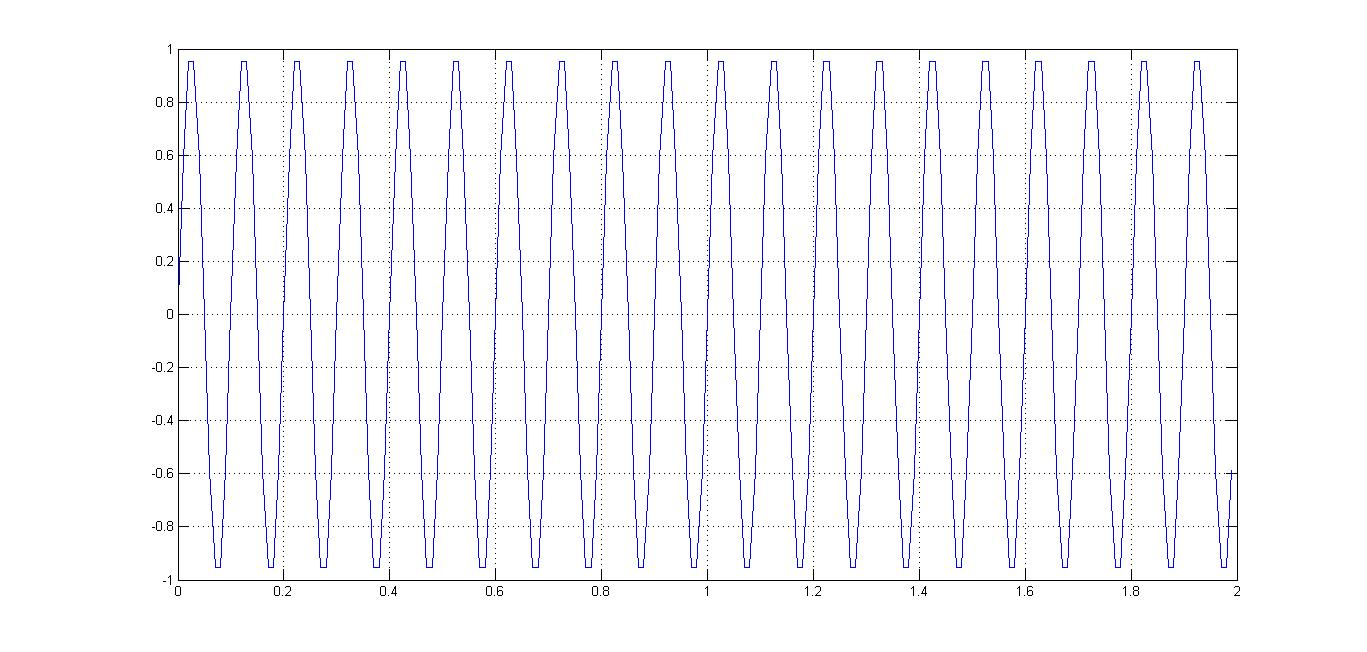
\includegraphics[angle=0, scale = 0.3]{sint.jpg}
рис. 1 Временная характеристика чистого синусоидального сигнала
\end{center}
\begin{center}
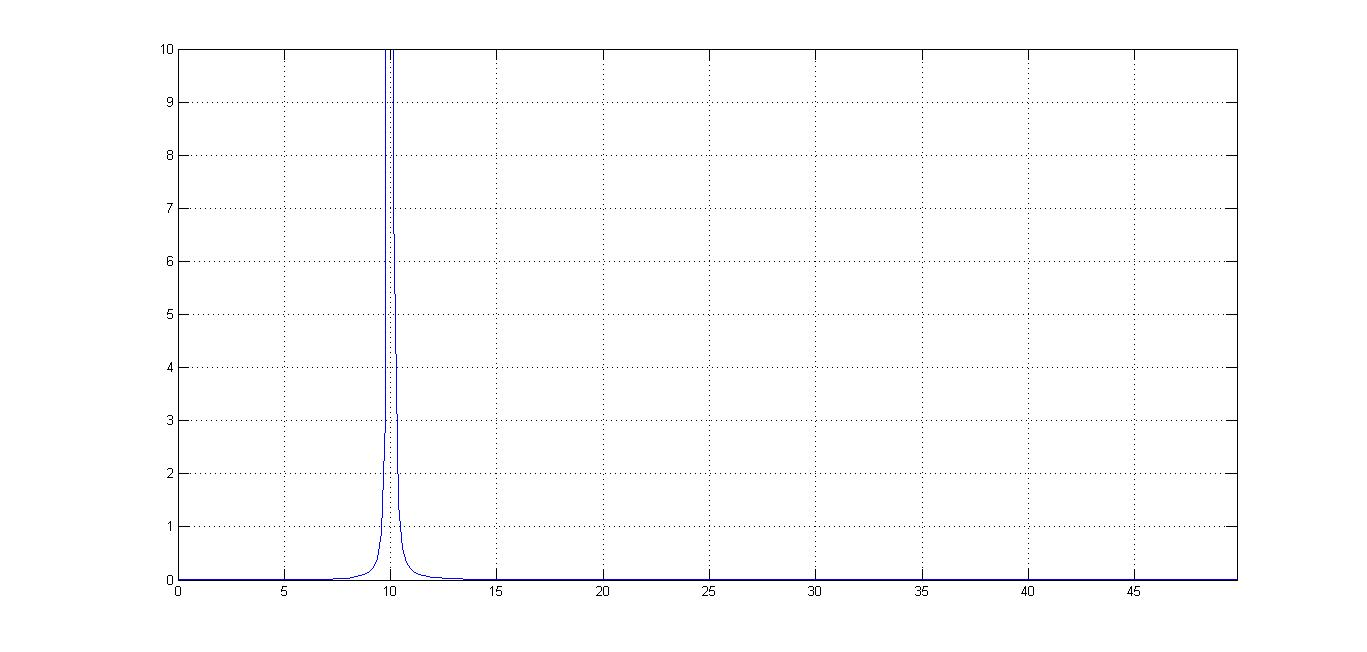
\includegraphics[angle=0, scale = 0.3]{sinch.jpg}
\end{center}
рис. 2. Частотная характеристика чистого синусоидального сигнала
\end{figure}
\begin{figure}
\begin{center}
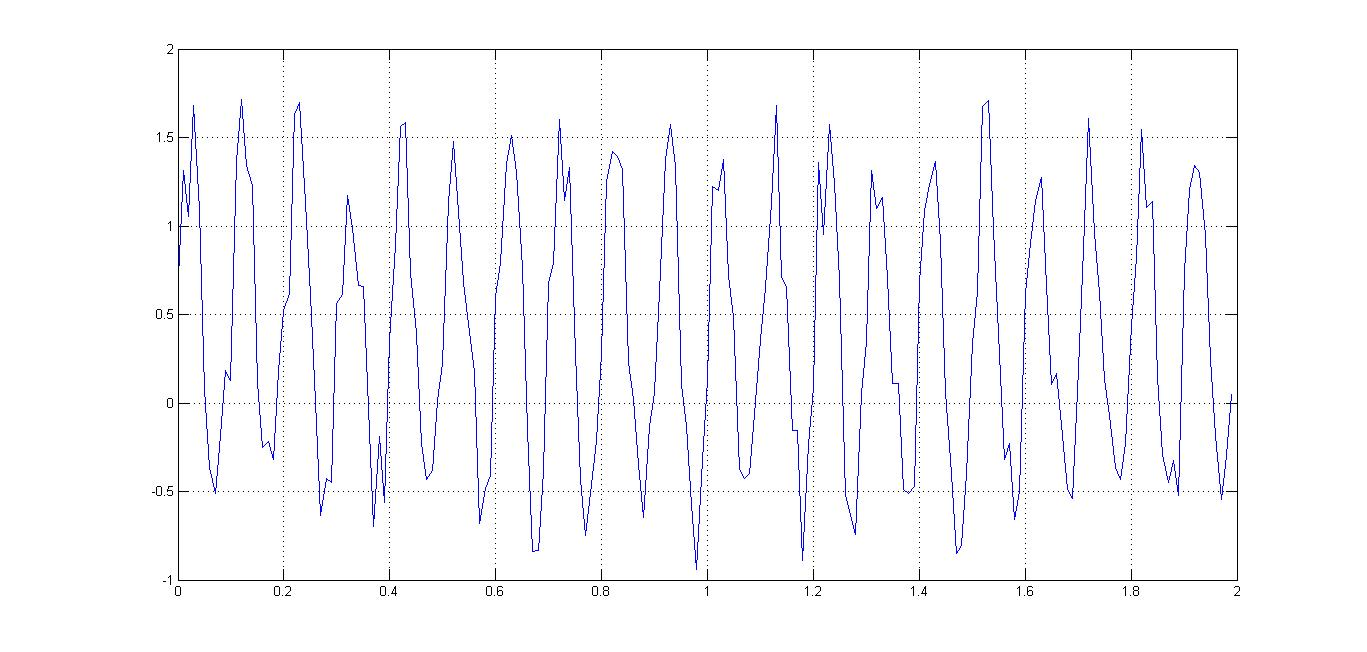
\includegraphics[angle=0, scale = 0.3]{nsint.jpg}
\end{center}
рис. 3. Временная характеристика зашумленного синусоидального сигнала
\begin{center}
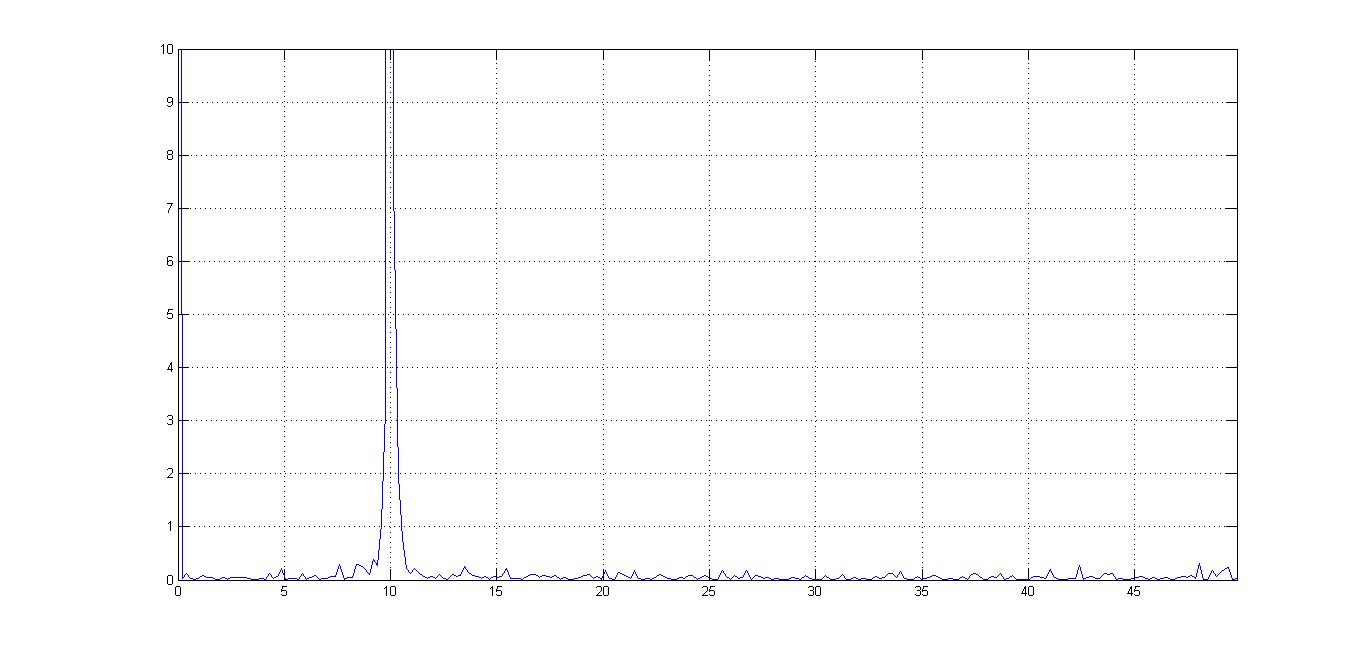
\includegraphics[angle=0, scale = 0.3]{nsinch.jpg}
\end{center}
рис. 4. Частотная характеристика зашумленного синусоидального сигнала
\end{figure}
Как видно из графиков, регулярная составляющая, как у чистого синусоидальног осигнала, так и у зашумленного равна 10Гц. Временная же характеристика чистого и зашумленного сигнала отличается достаточно сильно, хотя в обоих случаях заметны общие черты.
\section{Вывод}
Данная лабораторная работа заключалась в получении и сравнении спектров чистого и зашумленного сигнала. Спектры сигналов вычислялись на ограниченном промежутке. Для этого длина промежутка и частота квантования выбирались так, что бы результаты вычислений были достаточно точными. Полученные значения совпали с ожидаемыми. Стоит отметить, что спектр получается периодическим по частоте. Это вызвано тем, что при разложении сигнала в ряд Фурье, он умножается на комплексную экспоненту, которая обладает свойством периодичности.
\chapter{Лабораторная работа 5}
\section{Цель работы}
Целью данной работы является получение представлений о свойствах спектров, а именно:
\item Построение полигармонического сигнала
\item Построение прямоугольного импульсного сигнала
\item Построение треугольного импульсного сигнала
\item Получение спектров этих сигналов
\item Создание моделей в Simulink
\section{Теоритическая часть}
В данной работе мы рассматриваем три типа сигналов: полигармонический, прямоугольный импульсный и треугольный. Их формулы представленны ниже:
\item полигармонический сигнал 
\begin{displaymath}
y(t) = \sum_{n=0}^N-1 cos(nt)
\end{displaymath}
\item прямоугольный импульсный сигнал
\begin{displaymath}
y(t) = \Pi (t,T_i)
\end{displaymath}
\item треугольный импульсный сигнал
\begin{displaymath}
y(t) = \Delta (t,T_i)
\end{displaymath}
Для получения треугольного сигнала используется операция свертки двух прямоугольных сигналов, производимая по формуле:
\begin{displaymath}
(f*g)(x) = int_inf^-inf f(y)g(x-y)dy
\end{displaymath}
\section{Код matlab}
x = 0:0.01:4*pi;
f0=5;
y = 0;
for i=0:1:100
    y = y + cos(i*x);
end 
plot(x(1:100),y(1:100))
grid
figure
spectrum = fft(y,512);
norm_spectrum = spectrum.*conj(spectrum)/512;
f=100*(0:255)/512;
plot(f, norm_spectrum(1:256))
axis([0 max(f) 0 10])
grid
figure
y1 = square(x,50);
plot(x(1:1000),y1(1:1000),'LineWidth',2);
ylim([-1.2,1.2]);
grid
figure
spectrum = fft(y1,512);
norm_spectrum = spectrum.*conj(spectrum)/512;
f1=100*(0:255)/512;
plot(f1, norm_spectrum(1:256))
axis([0 max(f1) 0 10])
grid
figure
y2 = conv(square(x,50),square(x,50));
plot(x(1:1000),y2(1:1000),'LineWidth',2);
grid
figure
spectrum = fft(y2,512);
norm_spectrum = spectrum.*conj(spectrum)/512;
f2=100*(0:255)/512;
plot(f2, norm_spectrum(1:256)/1000)
axis([0 max(f2) 0 50])
grid
\section{Результаты работы}
В результате, были полученны 6 графиков: графики полигармонического, прямоугольного и треугольного сигналов, а так же графики их спектров соответственно. Графики представлены на рисунках ниже.
\begin{figure}
\begin{center}
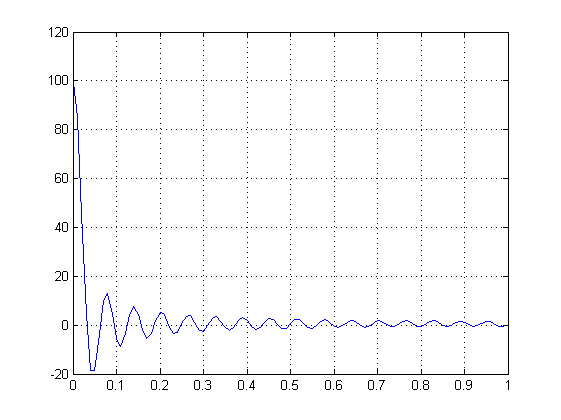
\includegraphics[angle=0, scale = 0.9]{5_1.png}\newline
рис. 5. Полигармонический сигнал\newline
\end{center}
\end{figure}
\begin{figure}
\begin{center}
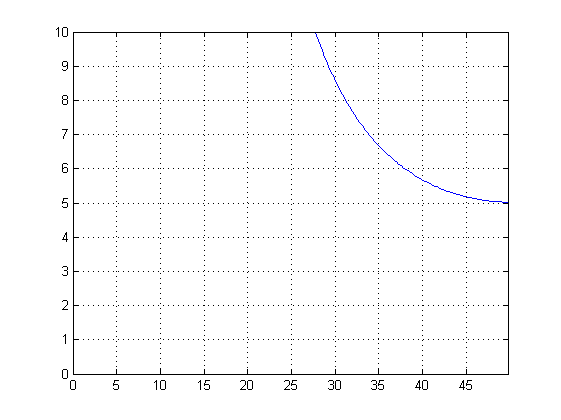
\includegraphics[angle=0, scale = 0.9]{5_2.png}\newline
рис. 6. Спектр полигармонического сигнала\newline
\end{center}
\end{figure}
\begin{figure}
\begin{center}
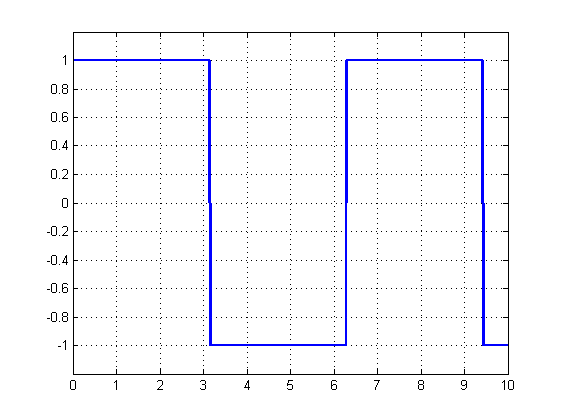
\includegraphics[angle=0, scale = 0.9]{5_3.png}\newline
рис. 7. Прямоугольный сигнал\newline
\end{center}
\end{figure}
\begin{figure}
\begin{center}
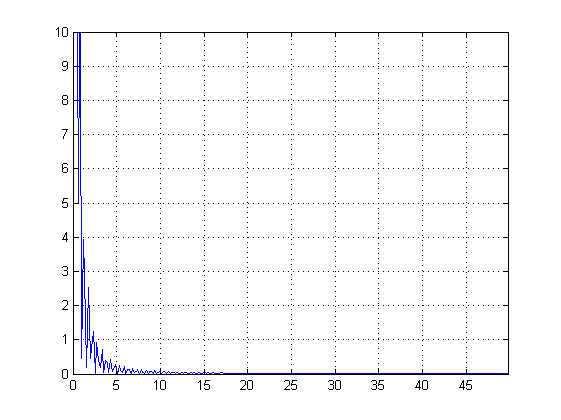
\includegraphics[angle=0, scale = 0.9]{5_4.png}\newline
рис. 8. Спектр прямоугольного сигнала\newline
\end{center}
\end{figure}
\begin{figure}
\begin{center}
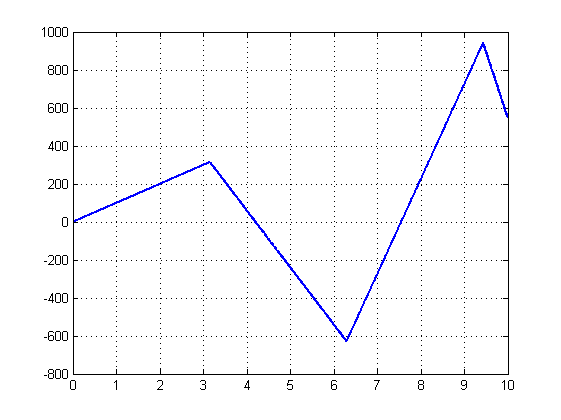
\includegraphics[angle=0, scale = 0.9]{5_5.png}\newline
рис. 5. Треугольный сигнал\newline
\end{center}
\end{figure}
\begin{figure}
\begin{center}
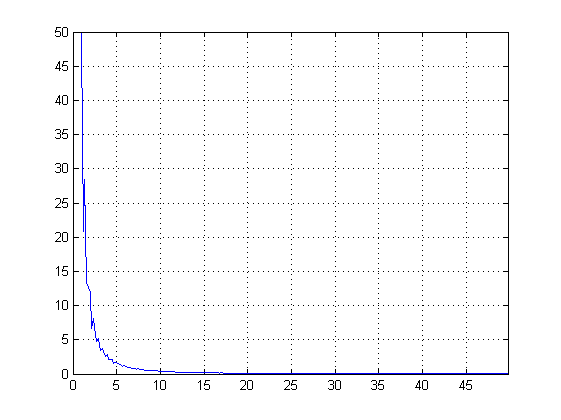
\includegraphics[angle=0, scale = 0.9]{5_6.png}\newline
рис. 5. Спектр треугольного сигнала\newline
\end{center}
\end{figure}
\end{document}
\section{Вывод}
В данной лабораторной работе было проведено моделирование основных видов сигналов: полигармонического, прямоугольного и треугольного, а так же были получены их спектры. Сигналы были полученны как при помощи формул данных функций, так и при помощи среды моделирования Simulink. Спектры сигналов так же были получены обоими вышеприведенными способами. Стоит отметить получение треугольного сигнала, т.к. он был получен не при помощи конкретной формулы, а путем свертки двух прямоугольных сигналов. Это возможно из-за того, что линейная функция может быть полученна как интеграл от двух констант. Таким образом, мы получаем две линейные функции, с отличием в коэфициенте наклона (у одной он положителен, а у другой отрицателен). Так же стоит отметить, что все полученные результаты соответствуют теоретическим ожиданиям.
